\section{FeatureSpy Design}
\label{sec:design}

We design \sysnameF with the following goals in mind.

\begin{itemize}[leftmargin=*]

\item {\bf Attack detection.} It reliably detects the learning-content attack against tampering by the client (i.e., robustness). Also, it achieves a high probability for catching the attack, while the number of misjudgements is small.
\item {\bf Confidentiality and bandwidth/storage efficiency.} It preserves source-based encrypted deduplication, so as to achieve  data confidentiality and bandwidth/storage efficiency. Also, it mitigates the information leakage due to key compromise.
\item {\bf Low performance overhead.} It detects the learning-content attack in the write path, and incurs low performance overhead in encrypted deduplication deployment.
\item {\bf Limited trusted computing base (TCB).} It manages minimal trust portions and function call interfaces for the SGX enclave; this is a necessary design goal in light of abusing interface function calls \cite{lie05}.
\end{itemize}

We first present a strawman (insecure) design to demonstrate how we detect the learning-content attack by monitoring  content processing. Then, we present \sysnameF, which prevents a malicious client from bypassing the attack detection procedure.



\subsection{Strawman Design}
\label{sub:basic}

\paragraph{Overview.} Our insight is that the adversary that launches the learning-content attack enumerates many {\em similar} chunks, which follow identical content patterns with information changes in a few  regions. In other words, such chunks are likely to share the same {\em content features} (that can be generated based on the corresponding chunk contents via {\em N-transform} \cite{shilane12}, see a latter part ``features extraction'' of this subsection), and be  processed within a small time window. This leads to a {\em skew feature distribution} for each time window in the attack procedure, since some features are shared by most of the chunks that are processed together.

On the other hand, we argue that the feature distribution of consecutive chunks (that are processed together \cite{zhu08}) in real-world untampered storage workloads is generally {\em uniform} (i.e., different features correspond to the same number of chunks).
Specifically, we analyze two real-world datasets (see \S\ref{sub:datasets} for dataset details), and partition the stream of chunks in each dataset into multiple non-overlapped windows, such that each window includes $W$ consecutive chunks. We extract three ordered features for each chunk via N-transform \cite{shilane12}. For each window, we count the {\em normalized difference} (i.e., the absolute difference divided by the total number of chunks in the window) between the maximum and minimum numbers of chunks that share an identical $i$-th feature ($i=1, 2$ and $3$). A lower normalized difference of a window indicates that the corresponding feature distribution is more uniform.


Figure~\ref{fig:featureDistribution} presents the normalized differences of all windows (with the sizes of $W$ = 1\,K, 5\,K, and 10\,K, respectively) based on their first features (i.e., $i$ = 1). The results for the other features are similar, since features across different orders are unlikely to be identical (due to the principle of N-transform); hence we omit them here.
We observe that although the distribution of the normalized differences across different windows is skew, each window only has a small value (e.g., up to 0.035 in Linux and 0.005 in CouchDB) of normalized difference. When $W$ = 1\,K, 5\,K and 10\,K, the features are even shared by an identical number of chunks (i.e., uniform feature distribution) in 91.5\%, 58.3\% and 29.9\% CouchDB windows, respectively.


\begin{figure}
  \centering
  \begin{tabular}{cc}
    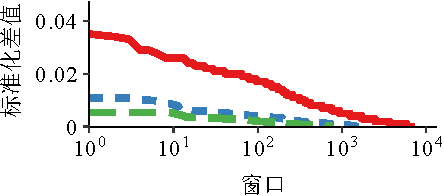
\includegraphics[width=1.55in]{pic/featurespy/plot/featureDistribution/featureDistributionLinux.pdf} &
                                                                                            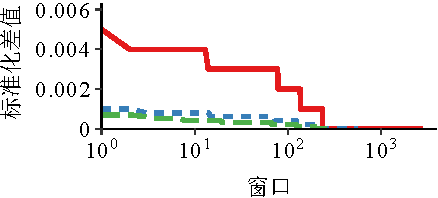
\includegraphics[width=1.55in]{pic/featurespy/plot/featureDistribution/featureDistributionCouchbase.pdf} \\
    {\small (a) Linux} & {\small (b) CouchDB} \\
    \end{tabular}
  \vspace{-6pt}
  \caption{Normalized differences across different windows in two real-world datasets. The windows in the x-axis are sorted by their normalized differences.}
  \label{fig:featureDistribution}
  \vspace{-6pt}
\end{figure}


Thus, the strawman design detects the learning-content attack by {\em differentiating feature distributions}. Figure~\ref{fig:architecture}(a) presents the architectural workflow of the strawman design.
Since \sysnameF is co-located with the client that may tamper with unprotected memory, it protects the feature extraction and attack detection procedures via the SGX enclave, so as to honestly report the attack event. Specifically, it enters the enclave to extract the content features of each plaintext chunk and reports an attack if many chunks match identical content features (i.e., similar). If no attack is announced, it continues to perform source-based encrypted deduplication (\S\ref{sub:basics}). In the following, we address the design details.

%(note that we do not choose to protect all client-side operations via the enclave, due to the huge TCB

% Thus, we propose to differentiate normal and attack cases by examining feature distributions. Specifically, we monitor the processing of chunks, compare the content features of each chunk, and report an  attack event if the client inputs many  chunks that have identical features for processing.

%to be processed in a small time window.

\paragraph{Features extraction.}
We extract the content features of each plaintext chunk via {\em N-transform} \cite{shilane12}, which is widely used to
detect chunk-level resemblances. N-transform is defined based on $N$ (e.g., 12 by default) pairs of coefficients $(a_i, m_i)$, where $N$ indicates how many {\em sub-features} (based on which N-transform generates features, see below) to be extracted for each chunk. Specifically, for each plaintext chunk $M$, it uses Rabin fingerprinting \cite{rabin81} to compute many fingerprints over the 32-byte sliding windows of chunk data, and transforms the Rabin fingerprint $fp$ in each sliding  window as:
\begin{eqnarray}
  \label{eq:feature}
  \pi_i = a_i * fp + m_i \mod 2^{32},
\end{eqnarray}
where $i$ = 1, 2,\ldots, $N$. It derives the $i$-th sub-feature of $M$ as $fp$, if $fp$ leads to the {\em maximum} $\pi_i$ among other Rabin fingerprints. The rationale is that changes in small regions are likely to affect some Rabin fingerprints, among which only a few (as the sub-features) generate the maximum values of $\{\pi_i\}$. Thus, the majority sub-features remain stable for similar chunks.

N-transform computes a feature by combining multiple (e.g., four by default) consecutive sub-features together. It characterizes each chunk by a set $S$ (e.g., by default the number of features $|S| = 3$) of features, in order to mitigate the computational overhead of comparing many sub-features for similarity detection. Specifically, the more common features two chunks have, the more likely to be similar they are.


\paragraph{Attack detection.}
We manage a hash table in the enclave to track how many plaintext chunks share identical content features. Each entry of the hash table maps a feature to the number of times (four bytes) that the feature occurs across different chunks.
 In addition,
we define a window size $W$ (e.g., 5\,K by default) and periodically clear all table entries per processing $W$ chunks, such that the hash table only keeps the {\em recent} occurrences of features in a short time. Note that the hash table is up to 5\,K $\times$ 3 $\times$ (16 bytes + 4 bytes) $\approx$ 300\,KiB and adds negligible memory overhead to the SGX enclave, where each chunk has three features, and each feature is concatenated from four sub-features that takes four bytes each according to the default configuration of N-transform.

To examine each plaintext chunk, we query the hash table based on {\em each} of its content features. If a feature does not exist, we add the feature  into the hash table, and initialize the corresponding occurrence with one; Otherwise if the feature exists, we increment the corresponding occurrence by one. We report an attack if the occurrence reaches a pre-defined ratio $T$ (e.g., 3\% by default) of the window size $W$.




\subsection{FeatureSpy Overview}
\label{sub:secure_design}

One security limitation of the strawman design is that it is vulnerable to {\em bypassing} the attack detection procedure (Figure~\ref{fig:architecture}(a)). Specifically, the malicious client can directly inject its self-constructed chunks to be processed by the unprotected operations (e.g., key generation), in order to launch the learning-content attack (\S\ref{sub:basics}).


%The question is how to design the SGX-based architecture of \sysnameF, such that it not only protects the attack detection operation via SGX, but also prevents the adversary from bypassing the detection procedure.


\begin{figure}
  \centering
  \begin{tabular}{c}
    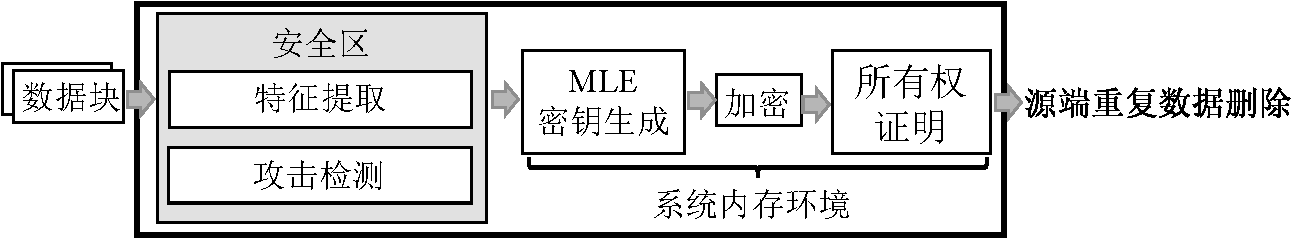
\includegraphics[width=3.25in]{pic/featurespy/naive.pdf} \\
    {\small (a) Strawman design} \vspace{5pt}\\
    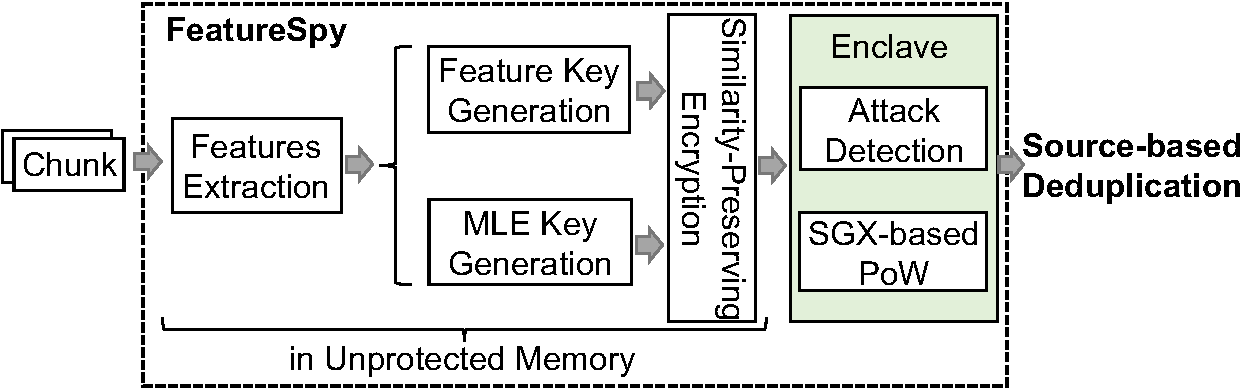
\includegraphics[width=3.25in]{pic/featurespy/architecture.pdf} \\
    {\small (b) Secure design}
  \end{tabular}
  \vspace{-6pt}
  \caption{Architectural workflows of designs. The strawman design is vulnerable to bypassing the detection procedure. \sysnameF couples the attack detection procedure with SGX-based PoW \cite{ren21} in the enclave,  in order to prevent the bypassing.}
  \label{fig:architecture}
  \vspace{-6pt}
\end{figure}


\sysnameF builds on {\em SGX-based PoW} \cite{ren21} to prevent the client from escaping the detection procedure. Specifically, the SGX-based PoW approach \cite{ren21} takes each ciphertext chunk as input and enters the SGX enclave to compute the fingerprint of the ciphertext chunk, as well as a signature of the fingerprint. The cloud proceeds to check if the fingerprint corresponds to a stored ciphertext chunk (i.e., deduplication) only when the signature is successfully verified. Since the cloud responds based on {\em authenticated} fingerprints that are processed by the SGX enclave, a client cannot identify the existence of the chunks that it is unauthorized to access.

Thus, a na\"{i}ve approach is to enlarge the enclave in the strawman design to totally perform detection, key generation, encryption, and SGX-based PoW in the enclave. In this case, only the chunks processed by the procedures in the SGX enclave are accepted by the cloud for deduplication (due to SGX-based PoW), and the malicious client cannot bypass any procedure.
However, the approach incurs a huge TCB and introduces potential performance \cite{arnautov16, harnik18, dinhngoc19} and security \cite{lie05} issues.


\sysnameF proposes to {\em perform attack detection based on ciphertext chunks}, and couples only the detection procedure with SGX-based PoW in the enclave (Figure~\ref{fig:architecture}(b)), so as to reduce the size of TCB.

%SGX-based PoW is performed only on the ciphertext chunks, whose features are examined (in the attack detection procedure), such that a malicious client cannot bypass the detection procedure.

% The cloud responds only when the ownerships of the corresponding ciphertext chunks are successfully verified, such that a compromised client cannot identify the ciphertext chunks owned by other clients
% Since the deduplication patterns are only returned based on  the {\em examined} chunks by the detection procedure in the enclave, a compromised client cannot directly perform source-based deduplication based on
%  its self-constructed chunks  for bypassing the detection procedure.
% computes the fingerprint of each ciphertext chunk and generates a {\em signature} based on the fingerprint in the enclave, such that
% We  propose a {\em secure design} , which  couples
% Specifically, we now detect the learning-content attack based on ciphertext chunks (see below).
% If no exception is reported, the



\paragraph{Challenge.}
However, a new challenge is raised for {\em detecting similarity based on ciphertext chunks}, since the enclave now only views the encrypted data.  It is impossible to detect similarity after MLE, as MLE keys are derived from the {\em whole contents} of plaintext chunks (\S\ref{sub:basics}). This maps similar (but distinct) plaintext chunks to totally different ciphertext chunks, thereby destroying similarity.

% Recently, Wu {\em et al.} \cite{wu21} propose

% An alternative approach is {\em feature-based encryption (FBE)}, which performs encryption/decryption based on a key (called {\em feature key}) derived from the content features of each plaintext chunk. Since similar chunks only differ in a few data regions, they are likely to have the same feature key, and a number of common data blocks (each of which takes 16 bytes in AES) from the beginning of contents.
% Considering that encrypted deduplication \cite{douceur02, shah15} necessitate a fixed {\em initialization vector (IV)} (to preserve deterministic encryption),
% the first a few blocks in the corresponding ciphertext chunks are identical due to the {\em block-chaining property} of some popular block cipher modes (e.g., CBC and CFB \cite{dworkin01}), and similarity detection can be performed by examining such initial blocks (of each ciphertext chunk).


An alternative cryptographic primitive is {\em feature-based encryption (FBE)}, which performs encryption/decryption based on a key (called {\em feature key}) derived from the content features of each plaintext chunk.
Since similar chunks only differ in a few data regions, they are likely to  have the same feature key, and first a few data blocks (each of which takes 16 bytes in AES). Considering that  encrypted deduplication \cite{douceur02, shah15} necessitates a fixed {\em initialization vector (IV)} (to preserve deterministic encryption), FBE preserves the equality of the first a few data blocks of similar chunks (due to the {\em block-chaining encryption} property of the block cipher modes, such as {\em cipher block chaining (CBC)} and {\em cipher feedback (CFB)} \cite{dworkin01}), and similarity detection can be performed by comparing such data blocks in each ciphertext chunk.



% FBE supports to detect similar original plaintext chunks by comparing the first a few data blocks in the corresponding ciphertext chunks.
% FBE is likely to generate identical feature keys for similar plaintext chunks, and preserves similarity after encryption.
% For example, suppose that FBE uses the {\em ciphertext feedback  (CFB)} mode \cite{dworkin01} as the underlying encryption function. In addition to the symmetric key, the CFB mode encrypts the first block of each plaintext chunk based on an {\em initialization vector (IV)}, and each following block based on the ciphertext of the corresponding previous block. Considering that encrypted deduplication implementations \cite{douceur02, shah15} necessitate a fixed IV to preserve deterministic encryption, if two similar plaintext chunks (i.e., assigned with the same feature key) have $i$ common blocks from the beginning of contents, then the first $i$ blocks in the corresponding ciphertext chunks under the CFB mode are the same. It is feasible to detect similar plaintext chunks by examining the initial $i$ blocks of corresponding ciphertext chunks.


However, FBE is vulnerable to key compromise, since a feature key corresponds to a set of chunks that have identical content features. A malicious client can use its compromised feature keys to fully decrypt many chunks, even some of which are {\em beyond its access scope}.

% FBE is likely to generate identical feature keys for similar plaintext chunks, and preserves similarity after encryption.
% For example, suppose that FBE uses the {\em ciphertext feedback  (CFB)} mode \cite{dworkin01} as the underlying encryption function. In addition to the symmetric key, the CFB mode encrypts the first block of each plaintext chunk based on an {\em initialization vector (IV)}, and each following block based on the ciphertext of the corresponding previous block. Considering that encrypted deduplication implementations \cite{douceur02, shah15} necessitate a fixed IV to preserve deterministic encryption, if two similar plaintext chunks (i.e., assigned with the same feature key) have $i$ common blocks from the beginning of contents, then the first $i$ blocks in the corresponding ciphertext chunks under the CFB mode are the same. It is feasible to detect similar plaintext chunks by examining the initial $i$ blocks of corresponding ciphertext chunks.
% %the common initial {\em blocks} (each of which takes 16 bytes for AES) of such chunks under some block cipher modes.
% %For example, in addition to the symmetric key,



This poses a dilemma in choosing a proper cryptographic primitive: MLE is robust against key compromise (i.e., a compromised MLE key cannot  be used to decrypt other chunks except the corresponding one) but destroying similarity, while FBE preserves the similarity of original chunks but vulnerable to key compromise.



\subsection{Similarity-preserving Encryption}
\label{sub:spe}


We propose {\em similarity-preserving encryption (SPE)}, which builds on the MLE key and the feature key, simultaneously, in order to mitigate key compromise via the MLE key while preserving similarity via the feature key.
Specifically, due to the limited content differences of similar chunks, SPE samples a small part (e.g., the first 32 bytes that take 0.4\% of an 8\,KiB chunk) from each plaintext chunk, called the {\em similarity indicator}, such that the similarity indicators of similar chunks are likely to be the same. It encrypts the similarity indicator of each plaintext chunk with the corresponding feature key, while the remaining large part (that takes 99.6\% of an 8\,KiB chunk) of chunk content with the MLE key. Then, we can  detect similarity based on ciphertext chunks by verifying if the corresponding (encrypted) similarity indicators (e.g., the first 32 bytes of each ciphertext chunk) are identical.
Note that SPE does not degrade the storage efficiency of cross-user encrypted deduplication (\S\ref{sub:basics}), since identical chunks share the same content features (and hence feature keys) and MLE keys.

We argue that SPE  mitigates the information leakage of FBE against key compromise. The insight is that the feature key of a compromised chunk $M$ can only be used to decrypt the similarity indicators of the  chunks similar to $M$. However, since such chunks are likely to have the same similar indicator with $M$, SPE does not incur additional information leakage. Even a rare chunk (that is similar to $M$) has a different similarity indicator, the information leakage is dramatically reduced compared to FBE, and subject to the size of the similar indicator.
In the following, we present the design details of how we generate the feature key for SPE.




% SPE encrypts a small part (called {\em similarity indicator} that 32 bytes or 0.3\% of an 8\,KiB chunk) of each plaintext chunk with the feature key while the remaining large part (called {\em trimmed chunk} that takes 99.6\% of an 8\,KiB chunk) of the chunk content with the MLE key.
% Due to the limited content differences of similar chunks,  are likely to also have the same indicator due to their limited differences on chunk contents.
% it is feasible to
% Since similar chunks have a large fraction of duplicate content, they are likely to have the same indicator in addition to the feature key.
% since similar chunks only differ in a few regions,  we can sample
% Thus, we
% We can detect similarity based on ciphertext chunks by verifying if the corresponding (encrypted) indicators are identical. Specifically,
%  \sysnameF now tracks the occurrences of indicators (rather than features in the strawman design in \S\ref{sub:basic}), and reports an exception if the occurrence of some indicator exceeds a pre-defined ratio of the window size (\S\ref{sub:basic}). In addition, since the remaining large part is protected by the MLE key, the information leakage due to key compromise is subject to the size of the indicator.
% Note that SPE does not degrade the storage efficiency of cross-user encrypted deduplication (\S\ref{sub:basics}), since identical chunks share the same content features (and hence feature keys) and MLE keys.
% In the following, we address how the feature key is derived for SPE.




%We propose {\em similarity-preserving encryption (SPE)}, which builds on the MLE key and the feature key, simultaneously, such that it can mitigate key compromise via the MLE key while preserving similarity via the feature key.
%In the following, we present how we generally derive the feature key, followed by the SPE design.
% which augments MLE with similarity preservation while mitigating the key compromise of FBE. Our idea is to  Specifically, since similar chunks only differ in a few regions,  we can sample a small part  in a fixed position (e.g., in the beginning of chunk content), called , such that the indicators of similar chunks  are likely to be the same. Thus, we encrypt the indicator of each plaintext chunk with its feature key, while
%  Specifically,
%  \sysnameF now tracks the occurrences of indicators (rather than features in the strawman design in \S\ref{sub:basic}), and reports an exception if the occurrence of some indicator exceeds a pre-defined ratio of the window size (\S\ref{sub:basic}). In addition,
%preserves similarity via the feature key while builds on the MLE key to mitigate the leakage of sensitive information against key compromise.



\paragraph{Feature key generation.}
Recall that we extract three content features for each plaintext chunk via N-transform (\S\ref{sub:basic}), and a basic key generation approach (called {\tt allFeature}) is to concatenate all features, and compute the feature key based on the cryptographic hash of the concatenation result. However, {\tt allFeature} fails to generate identical feature keys for many similar chunks. Specifically, if the content difference of the similar chunks is exactly in the sliding window that yields a sub-feature (\S\ref{sub:basic}), the chunks will have distinct feature keys, and it is impossible to detect the similarity between them even if the remaining original contents are identical.

We build on the {\em sampling-based approach} \cite{bhagwat09, dong11, qin17} to relax the key generation criteria. The idea is to sample a {\em representative} feature for each plaintext chunk, and compute the feature key based on the sampled feature. This tolerates content differences, and generates identical feature keys for a wide range of plaintext chunks.

We consider two ways to choose the representative feature. Specifically, {\tt firstFeature} generates a feature key based on the {\em first} feature of each plaintext chunk. The advantage is that we do not need to compute subsequent sub-features and features (\S\ref{sub:basic}), and mitigate the computational overhead \cite{zhang19} of N-transform.

We also consider {\tt minFeature}, which builds on {\em Broder's theorem} \cite{broder97} to generate the feature key based on the {\em minimum} feature (i.e., have the minimum value in all features) of each plaintext chunk. Specifically, Broder's theorem states that if two plaintext chunks have many common features (i.e., similar with a high probability), they are likely to share the same minimum feature. That is:
\begin{eqnarray}
  \label{eq:broder}
 \Pr[\min(S_1) = \min(S_2)] = \frac{|S_1 \cap S_2|}{|S_1 \cup S_2|},
\end{eqnarray}
where $S_i$ is the set of features for a plaintext chunk $M_i$, and $\min(S_i)$ returns the minimum value of the features in the set $S_i$ ($i = 1, 2$). Thus, {\tt minFeature} tends to generate identical feature keys for the highly similar chunks. In \S\ref{sec:evaluation}, we will study the trade-off of different key generation approaches of SPE.

Note that in addition to working on features, an alternative design is to generate a feature key based on the first or the minimum {\em sub-feature}. We do not choose this design, due to the low entropy of a sub-feature. According to the original configuration \cite{shilane12} of N-transform, each sub-feature has only four bytes, and an adversary can efficiently launch the brute-force attack by  enumerating all possible sub-features/keys (up to $2^{32}$). On the other hand, in \S\ref{sec:implementation}, we re-configure N-transform to ensure that the key space based on features is large enough (e.g., $2^{256}$) against the brute-force attack.


% \paragraph{SPE design.}
% The basic idea is to sample a small part (e.g., 32 bytes or 0.39\% of an 8\,KiB chunk), as the {\em similarity indicator}, of each plaintext chunk, and encrypt the small part with the feature key while the remaining large part (called {\em trimmed chunk} that takes 99.61\% of an 8\,KiB chunk) of chunk content with the MLE key. It is feasible to detect similarity based on ciphertext chunks by verifying if the corresponding (encrypted) indicators are identical.
% Our insight is that if some bytes (e.g., public content patterns) are shared by many chunks, then such bytes are likely to be {\em non-sensitive}. Thus, the idea of SPE is to build on a few non-sensitive bytes to expose the similarity of original plaintext chunks, while preserving high security (i.e., against key compromise) of the remaining sensitive contents.
% Basically, it encrypts a small part , called the {\em indicator}, of each plaintext chunk with the feature key, while the . It can
% However,
% Also, since the remaining large part is protected by the MLE key, the information leakage due to key compromise is subject to the size of the indicator.
% Figure~\ref{fig:encryption} presents the design of SPE. Instead of using the output of the key generation instances (e.g., {\tt allFeature}, {\tt firstFeature} and {\tt minFeature}) to encrypt the indicator, it computes the feature key as the cryptographic hash of the concatenation of the and the indicator. It then
% Specifically, we sample a small part (e.g., 32 bytes or 0.39\% of an 8\,KiB chunk) from each plaintext chunk in a fixed position (e.g., in the beginning of the chunk content), called the {\em indicator}, and protect the indicator of each plaintext chunk with its feature key, while the remaining large part (that takes 99.61\% of an 8\,KiB chunk) of the chunk content with the MLE key. We can detect similarity based on ciphertext chunks by verifying if the corresponding (encrypted) indicators are identical.
% \begin{figure}
%   \centering
%   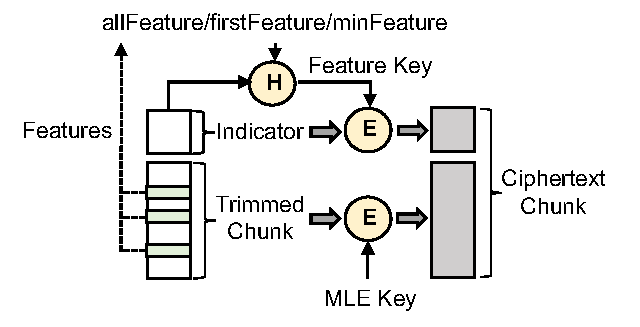
\includegraphics[width=3in]{pic/featurespy/encryption.pdf}
%   \vspace{-6pt}
%   \caption{Design of SPE. $\mathbf{H}(\cdot)$ and $\mathbf{E}(\cdot)$ are the hash and encryption functions, respectively.}
%   \vspace{-6pt}
%   \label{fig:encryption}
% \end{figure}
% since similar chunks only differ in a few regions,  such that the indicators of similar chunks  are likely to be the same (i.e., non-sensitive). Thus, we
% , which augments MLE with similarity preservation while mitigating the key compromise of FBE. Our idea is to build on the MLE key and the feature key, simultaneously, such that we can mitigate key compromise via the MLE key while preserving similarity via the feature key. Specifically,
%  \sysnameF now tracks the occurrences of indicators (rather than features in the strawman design in \S\ref{sub:basic}), and reports an exception if the occurrence of some indicator exceeds a pre-defined ratio of the window size (\S\ref{sub:basic}). In addition, since the remaining large part is protected by the MLE key, the information leakage due to key compromise is subject to the size of the indicator.
% Note that SPE does not degrade the storage efficiency of cross-user encrypted deduplication (\S\ref{sub:basics}), since identical chunks share the same content features (and hence feature keys) and MLE keys.
% In the following, we address how the feature key is derived for SPE.







%In \S\ref{subsub:secure_details}, we show how we can further enhance the protection of the indicator against key compromise.
%  presents the architecture of \sysnameF. It processes plaintext chunks in unprotected memory to extract features, generate keys and perform chunk-based encryption. In the SGX enclave, it performs attack detection, followed by PoW, such that the source-based deduplication is applied on the chunks that have been processed by the enclave.
% Figure~\ref{fig:architecture}(b) presents the architectural workflow of the secure design, which generates feature keys and MLE keys to perform SPE. In In the following,
% \paragraph{Similarity-preserving encryption.}
% We choose the indicator as the first $L$ bytes of each plaintext chunk.
% Figure~\ref{fig:encryption} presents the workflow of the similarity-preserving encryption, which combines FBE and MLE to preserve similarity after encryption (\S\ref{subsub:secure_idea}). Instead of directly encrypting the indicator with the feature key, we now hash the concatenation of the indicator and the feature key to form a hash key, and further use the hash key to encrypt the indicator. Our rationale is to ensure that a compromised feature key is insufficient to decrypt the indicator. Also,
% Specifically, the the feature key and the MLE key as input.

% \begin{figure}
%   \centering
%   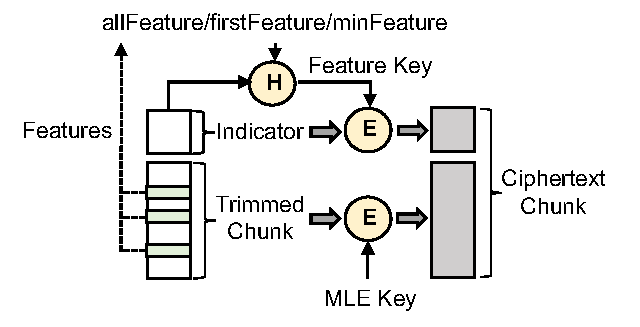
\includegraphics[width=3in]{pic/featurespy/encryption.pdf}
%   \vspace{-5pt}
%   \caption{Similarity-preserving encryption. $\mathbf{H}(\cdot)$ is a cryptographic hash function, and $\mathbf{E}(\cdot)$ is an encryption function.}
%   \vspace{-5pt}
%   \label{fig:encryption}
% \end{figure}


\subsection{Security Discussion}
\label{sub:security}

We discuss the confidentiality of \sysnameF (in particular SPE, which is the underlying encryption primitive), followed by its robustness against a malicious client.

\paragraph{Confidentiality against a compromised cloud.}
We have discussed the security improvement of SPE over FBE when keys are compromised (\S\ref{sub:spe}), and now
focus on the case that the keys remain secure. Our goal is to show that SPE preserves the security of encrypted deduplication against a compromised cloud. Specifically,
since SPE performs encryption via both MLE and FBE, its security is reduced to those of MLE and FBE. The previous work \cite{bellare13a} has shown
that MLE ensures that any  polynomial-time adversary cannot distinguish the ciphertext of a plaintext chunk from a random value (i.e., PRV\$-CDA), when the plaintext chunk is
drawn from a large space such that it is difficult to predict any chunk chosen from the space (i.e., {\em unpredictable}). In the following, we (informally) show that FBE preserves the security  of MLE if features are unpredictable.


We consider FBE as a generic form of MLE. If we treat the sampled feature(s) (e.g., the representative feature for {\tt firstFeature} and {\tt minFeature}, and all features for {\tt allFeature}) as a message $M$, then FBE actually uses the cryptographic hash of $M$ to encrypt the corresponding expansion $f(M)$ (i.e., plaintext chunk), where $f(\cdot)$ is an expansion function. Since each $M$ is unpredictable, the secret key  remains confidential against a polynomial-time adversary. Then, an adversary cannot distinguish a ciphertext from a random value, if the underlying symmetric encryption is secure.

% In addition, SPE performs encryption via both FBE and MLE, and hence its security relies on the primitives. Specifically, assuming the existence of an adversary that breaks SPE  with an advantage $\epsilon$, by triangle inequality, one can construct either an adversary that breaks either FBE  or MLE with an advantage at least $\epsilon/2$.

%{\bf TODO: Pls add informal security analysis here}
% First we note that the FBE is slightly different from MLE, in the sense that it uses the hash value of the sampled feature rather than the plaintext as a secret key, while this does not spoil the privacy due to the following reason. Since the plaintext chunks can be treated as (expanded) information on the feature, an FBE is essentially an MLE encrypting related information on a message (which is the feature in our case) embedded into the secret key, rather than encrypting the message itself. One can see that the MLE instantiated by Bellare et al. \cite{bellare13a} can do this without loosing privacy: as long as the feature is unpredictable, the secret key remains hidden and thus an adversary cannot distinguish a ciphertext from randomness due to the security of the underlying symmetric encryption. Therefore, the adversary learns little information on the plaintext chunks encrypted by the FBE.
% %Assuming that the feature is unpredictable, any polynomial-time adversary learns little information on the feature key and thus unable to distinguish a ciphertext of the FBE scheme from randomness.
% Moreover, the rest plaintext chunks encrypted by the MLE are only dependent of the MLE ciphertexts and the feature keys, while neither benefits the adversary due to the security of the MLE scheme and the unpredictability of the feature.
% As a result, the resulting SPE remains confidential under the security of the underlying FBE and MLE.


% Notice that in our case, we use the MLE scheme in a slightly different way, in the sense that we sometimes use the hash value of the sampled feature as a secret key, while this does not spoil the privacy. One can see that the sampled feature is unpredictable and the plaintext chunks can be treated as (expanded) information on the feature. Therefore, our scheme remains confidential as long as the MLE scheme can encrypt information on a message embedded into the secret key (rather than the message itself) without loosing privacy. This is the case for the instantiations in \cite{bellare13b}. The security proof proceeds in exactly the same way as the original one in [Appendix B]\cite{bellare13b} except for changing "$\mathcal{SE}(\mathbf{L}[i],\mathbf{M}[i])$" to "$\mathcal{SE}(\mathbf{L}[i],f(\mathbf{M})[i])$" and letting the message distribution $\mathcal{M}$ additionally outputs $f(\mathbf{M})$, where $f$ is an arbitrary polynomial-size function and $f(\mathbf{M})$ can be treated as arbitrary information on the hashed message. We refer the reader to [Appendix B]\cite{bellare13b} for the detailed proof.

% We further argue that while a sampled feature key might be dependent of  other plaintext chunks encrypted in a "standard way" by using the original MLE scheme, an adversary obtains no additional advantage on this, since the feature is unpredictable and thus its ciphertext reveals no information on other chunks.

Note that our informal analysis relies on the security assumption that the features are unpredictable, while we can mitigate the unpredictable assumption via server-aided key generation \cite{bellare13b} (see \S\ref{sec:implementation} for how we deploy \sysnameF in an existing encrypted deduplication system that addresses the unpredictable assumption).

%In \S\ref{sec:implementation}, we show how we integrate our design into an existing encrypted deduplication system \cite{ren21}.


% \subsubsection{Confidentiality}
% The confidentiality of our scheme is protected by the underlying MLE scheme instantiated with a symmetric encryption and a hash function as in \cite{bellare13b}. Recall that in an MLE scheme, a secret key is a hash value of the plaintext. The privacy (against chosen-distribution attacks) of an MLE scheme says that any polynomial-time adversary cannot distinguish honestly generated ciphertexts of unpredictable plaintexts from randomness, which provides us with confidentiality. Assuming that the hash function is modeled as an ideal one (i.e., a random oracle), for any adversary $\mathcal A$, there must exist polynomial-time adversaries $\mathcal B_1$ and $\mathcal B_2$ such that
% $$
% \mathbf{Adv}_{\mathcal A}^{prv-cda}\leq qm\cdot \mathbf{Adv}_{\mathcal B_1}^{kr}+2\cdot \mathbf{Adv}_{\mathcal B_2}^{ror}+\frac{4m^2}{2^k}+\frac{qm}{2^\mu}.
% $$
% Here, $q$ is the number of queries made to the hash function, $\mu$ is the min-entropy of the plaintext, $m$ is the number of plaintexts, $\mathbf{Adv}_{\mathcal A}^{prv-cda}$ is the advantage of ${\mathcal A}$ in breaking the privacy of the MLE scheme,
% and $\mathbf{Adv}_{\mathcal B_1}^{kr}$ and $\mathbf{Adv}_{\mathcal B_2}^{ror}$ are respectively the advantages of ${\mathcal B_1}$ and ${\mathcal B_2}$ in breaking the key recovery (KR) security and the one the one-time real-or-random (otROR) security of the symmetric key encryption scheme. Hence, if the underlying symmetric encryption scheme is simultaneously KR and otROR secure, which is widely believed for the instantiations given in \cite{bellare13b}, our resulting protocol remains confidential.


\paragraph{Robustness against a malicious client.}
We have discussed that an adversary cannot bypass the detection procedure (\S\ref{sub:secure_design}), and now focus on the robustness against other malicious actions (\S\ref{sec:setting}).


\begin{itemize}[leftmargin=*]
\item  {\bf Case 1: Tampering with unprotected procedures.}
  \sysnameF protects the detection procedure via SGX, yet a malicious client can tamper with the unprotected procedures. It may manipulate the features, similarity indicators, and keys, in order to cheat \sysnameF.
  We argue that these manipulations do not help learn contents from the other honest clients that follow our design, since the manipulations lead to a distinct ciphertext chunk with that produced by SPE (applied by an honest client), even if the original plaintext chunks are the same. This {\em prohibits deduplication}, and the learning-content attack that relies on the leakage of deduplication patterns is impossible.



%  deduplication is now {\em disabled} between the target ciphertext chunk (that is generated by the honest client) and any tampered one. The learning-content attack




  % key generation and encryption procedures. It may manipulate the similarity indicators of plaintext chunks (e.g., swap the similarity indicators of different plaintext chunks) or randomize ciphertext chunks (e.g., perform encryption via random keys), in order to cheat \sysnameF.
  % Specifically, a honest client should perform SPE on real plaintext chunks, thereby prohibiting deduplication between the target ciphertext chunk of the honest client and any manipulated ciphertext chunk. Thus, the learning-content attack is impossible.
  % In other words, the malicious client cannot exploit the existence of ciphertext chunk, and the learning-content attack is impossible. The reason is that the manipulation of the above contents prohibits
% while the compromised client uses its artificial keys or contents. This prohibits deduplication  between the target ciphertext chunk of the honest client and any manipulated ciphertext chunk  generated by tampered operations, and hence the learning-content attack is impossible.

% \item {\bf Case 2: Crafting feature distributions.}
%   Since \sysnameF examines the feature distribution of each window of chunks, an adversary may craft chunks to make the feature distribution seem realistic. Specifically, to shield a group of $x$ similar faked chunks, it creates another $W/x - 1$ chunk groups, such that each group includes $x$ chunks that share identical features and the content features of the chunks across different groups are  totally different, where $W$ is the number of chunks in a processing window. It randomly places all (i.e., $W/x$ groups in total) chunks in the window, in order to flatten the overall feature distribution.
%   Our design  generally detects this action, since the maximum number of  chunks (that have identical features) in each group is subject to a threshold $T$ (\S\ref{sub:basic}). To escape detection, the only way is to only submit a few chunks  (i.e., $x < T$) that have identical features in each processing window, yet slowing down the attack.

\item {\bf Case 2: Tampering with data processing.}
  Since \sysnameF monitors data similarity in the granularity of each processing window, a malicious client may tamper with an in-processing data stream, and carefully insert similar chunks (for attack), such that each window just includes a small fraction of  the similar chunks.  Although \sysnameF cannot detect the attack in this case, we argue that it slows down the learning-content attack. For example, without \sysnameF, the malicious client can full fill each window with similar chunks (i.e., the number is $W$) for attack, yet \sysnameF ensures that it can submit up to $W \times T$ similar chunks (otherwise it is detected). The attack cost is reduced by $1 / T$ times. By configuring a small $T$, we can make the learning-content attack too expensive to be impractical; the trade-off is that the possibility of misjudgement (i.e., report an attack in a normal case) is increased.


  %Also, it is feasible to still detect the learning-content attack by configuring a small $T$, yet introducing possibilitis of false positives.
\end{itemize}



\paragraph{Limitation.}
\sysnameF detects the learning-content attack from each {\em independent} client. However, an adversary may compromise multiple clients to cooperatively launch the learning-content attack. Now the number of similar chunks uploaded by each client is greatly reduced, and \sysnameF may not effectively detect the exception. We pose the defense against the cooperative learning-content attack as our future work.


% can schedule each compromised client to upload a subset of faked chunks, and
%  \sysnameF prevents abusing deduplication patterns, but it cannot protect against the leakage of deduplication patterns. In other words, when performing source-based deduplication, an adversary can still use its fully accessible file to learn the information that if someone has uploaded the same file.
%  We pose the full protection of deduplication patterns as our future work.


% Our rationale is to ensure that only the ciphertext chunks examined by \sysnameF can be processed by source-based deduplication, so as to
% prevent the malicious client from  directly submitting the fingerprints that are generated by itself. Also, this
% mitigates the threat of using a fingerprint to convince the ownership of the corresponding ciphertext chunk \cite{halevi11, ren21}.



% We design \sysnameF to perform attack detection {\em based on ciphertext chunks} that will be directly processed by source-based deduplication, such that the adversary cannot bypass the detection procedure. However,

% \paragraph{Design challenge.}

% \paragraph{Main idea.}





% \paragraph{Na\"{i}ve approach.}





% \paragraph{Our approach.}

% To address this issue, our idea is to generate the secret key of each chunk {\em based on its features} (rather than the whole chunk content in MLE \cite{bellare13a}), such that similar chunks are likely to have identical secret keys. To perform encryption, we use a special {\em bloCk cipher mode} \cite{dworkin01} (e.g., the {\em ciphertext feedback (CFB) mode} by default, see \S\ref{sub:detection} for detailed properties), such that the $i$-th ($i>1$) ciphertext block of the resulting ciphertext chunk only depend on the secret key and each previous/current $j$-th original plaintext block, where $j$ = 1, 2, $\ldots$, $i$. In other words, if two similar plaintext chunks have $i$ common plaintext blocks in the beginning of contents, then the first $i$ ciphertext blocks in the  corresponding ciphertext chunks are identical (assuming that the similar plaintext chunks have the same key). Thus, \sysnameF examines a number of {\em prefix} bytes of each ciphertext chunk, and deduces that two plaintext chunks are similar if their ciphertext chunks share the same prefix bytes.
% Since similar chunks differ in a few regions that are unlikely to be just in the beginning of each chunk, \sysnameF can detect most of similar chunks and successfully report the attack with a high probability.




% \paragraph{Architecture.}
% Figure~\ref{fig:architecture}(b) presents the architecture of \sysnameF.

% Here, we adopt the {\em SGX-based PoW} approach \cite{ren21} to further process ciphertext chunks if no exception is detected. Specifically,


% \subsection{Key Generation}
% \label{sub:keygen}

% \sysnameF builds on N-transform \cite{shilane12} to extract features from plaintext chunks. We introduce N-transform, followed by how we generate keys based on the N-transform features.




% \paragraph{Key generation schemes.}


% \subsection{Attack Detection}
% \label{sub:detection}

% \sysnameF detects the learning-remaining-content attack by examining the ciphertext chunks that are encrypted by the {\em ciphertext-feedback (CFB) mode} \cite{dworkin01}.

% %We introduce the chaining-based block cipher mode, followed by our design details.


% \begin{figure}
%   \centering
%   \subfigure[Encryption]{
%     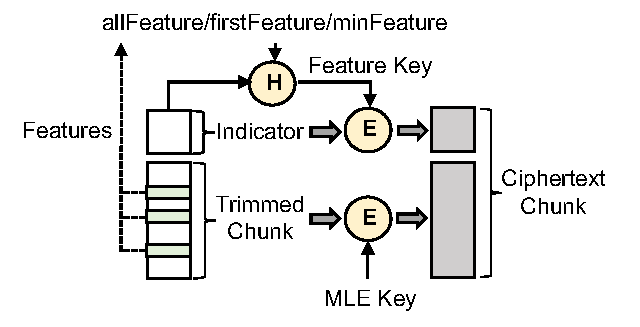
\includegraphics[height=.71in]{pic/featurespy/encryption.pdf}
%   }
%   \subfigure[Decryption]{
%     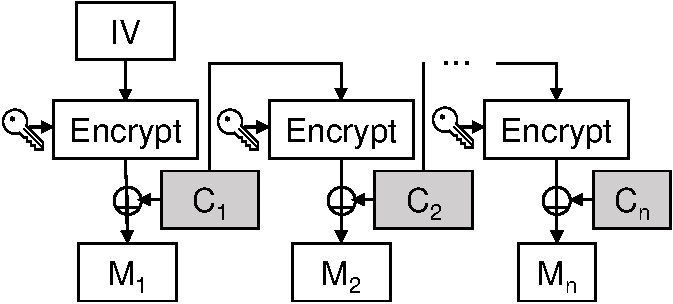
\includegraphics[height=.71in]{pic/featurespy/decryption.pdf}
%   }
%   \vspace{-5pt}
%   \caption{Encryption and decryption of CFB mode. The encryption of each block recursively depends on previous blocks. The last block that does not need to fit in the block size can still be processed without padding.}
%   \vspace{-5pt}
%   \label{fig:cfb}
% \end{figure}

% \paragraph{CFB mode.}
% The CFB mode extends block cipher to encrypt data that includes multiple blocks (e.g., each block has a fixed size of 16 bytes). Figure~\ref{fig:cfb} presents the encryption and decryption procedures of the CFB mode, which originally uses a freshly random {\em initialization vector (IV)} to process each chunk. We follow previous systems \cite{douceur02, shah15} to use a fixed IV, so as to enable encrypted deduplication.

% To encrypt a chunk $M$, the CFB mode first divides $M$ into $n$ blocks $M_1, M_2, \ldots, M_n$. To encrypt each block $M_i$, if $M_i$ is the first block (i.e., $i = 1$), it encrypts IV and XORs the encryption result with $M_1$: $C_1 = \mathbf{E}(K, IV) \oplus M_1$; otherwise if $M_i$ is not the first block (i.e., $i > 1$), it encrypts the previous ciphertext block $C_{i-1}$, and computes  $C_i = \mathbf{E}(K, C_{i-1}) \oplus M_i$, where $\mathbf{E}(\cdot)$ is the encryption function, $K$ is the feature-based key (\S\ref{sub:keygen}), and $\oplus$ is the bitwise XOR operation. To perform decryption, it recovers the first plaintext block as $M_1 = \mathbf{E}(K, IV) \oplus C_1$, and each following block as $M_i = \mathbf{E}(K, C_{i-1}) \oplus C_i$ ($i>1$). Since the encryption of each block in the CFB mode {\em recursively depends} on its previous blocks, we can
% examine the prefix bytes of ciphertext chunks to find similar original plaintext chunks (\S\ref{sub:overview}). Note that the {\em cipher block chaining (CBC)} and {\em output feedback (OFB)} modes also have the recursive dependency property, and fit our design.




% In addition to recursive dependency, our design choice is due to the {\em padding free} property of the CFB mode.
% If a chunk cannot be evenly dividible into blocks, the CFB mode does not need to pad the last block of the chunk to fit the block size. Instead, it cuts the encryption result (i.e., $\mathbf{E}(K, C_{n-1})$) of the penultimate ciphertext block into the same size of $M_n$ (Figure~\ref{fig:cfb}(a)), so as to enable the bitwise XOR operation (see above). This mitigates the management overhead of paddings, especially when processing  chunks that have varying sizes.

% \paragraph{Detailed design of attack detection.}



% % With a small $L$, it detects similar chunks even when the changes occur near the beginning of contents, but introduces more false positives, since the ciphertexts of unsimilar chunks may randomly share common prefix in a few bytes. With a large $L$, it achieves a high precision, yet cannot detect similar chunks, which differ in the first a few bytes. In Exp\#XXX, we will study the impact of different $L$.


% % examines similarity based on ciphertext chunks in the PoW enclave. Here, we choose to inspect the {\em $L$-byte prefix} (i.e., the first $L$ bytes, where $L$ = XXX by default) of each ciphertext chunk, and report an attack if many ciphertext chunks share the same $L$-byte prefix. The design rationality  is from two sides. On the one hand, similar chunks are likely to be encrypted with identical keys (see above), and their ciphertext chunks share the same $L$-byte prefix with a high probability (e.g., when the changes between similar chunks occur after the first $L$ bytes).
% % On the other hand, we cannot examine the subsequent blocks (in contrast to the prefix) of ciphertext chunks only, since they depend not only on the corresponding plaintext blocks and MLE key, but also on the previous plaintext/ciphertext blocks (e.g., the CBC encryption mode).
% % To detect the pattern-based attack, the PoW enclave

% \subsection{Security Discussion}
% \label{sub:security}
